\section{Results}

The main design goal of PIX is to produce efficient instrumented code. 
To investigate the efficiency of instrumented executables created by PIX, we ran several experiments 
on a selection of benchmarks from the the SPEC CPU2000 Integer benchmark suite comprised of
bzip2, crafty, gap, gzip, mcf, parser, perlmbk, twolf, vortex and vpr. All of the experiments are run on a
one core of a quad-core 2.4GHz IA32 Intel Xeon running Red Hat Linux Enterprise 4.1.2 (Linux kernel 2.6.18). 

The first set of experiments quantifies the overhead of the program relocation and 
transformation techniques used by PIX and
described in section \ref{Subsection:Relocation}. 
Recall that this technique adds an additional unconditional
branch execution to each function call in order to relocate the function, extends all of the branches in the code
to use 32-bit offsets, and pads each basic block whose size is fewer than 5 bytes with nops so that a
5 byte jump to the instrumentation code can be inserted. These transformations are performed on our benchmark set 
so that the code is ready for instrumentation but is not actually instrumented. 

Figure \ref{Figure:RelocOverhead} presents
the runtime overhead seen in the instrumentation-ready executables as a percentage of the original application runtime.
The figure shows that the maximum overhead due to these modifications is 6.5\%, with an
average overhead of just 1.6\%. Among a set of popular dynamic instrumentation toolkits,
Pin, DynamoRIO, Valgrind and Dyninst, the lowest overhead for running the application within the instrumentation
tool but performing no instrumentation
on the IA32 platform is obtained by using DynamoRIO. DynamoRIO has an average of 38\% overhead and a maximum overhead of 113\% on
our SPEC CPU2000 Integer benchmark set \cite{luk2005pin}. This shows that the 
relocation and transformation method used by PIX has a minimal
performance impact on the performance of these benchmarks and thus is a suitable approach as a basis for
producing efficient instrumented code.

\begin{figure}[ht]
\centering
\label{Figure:RelocOverhead}
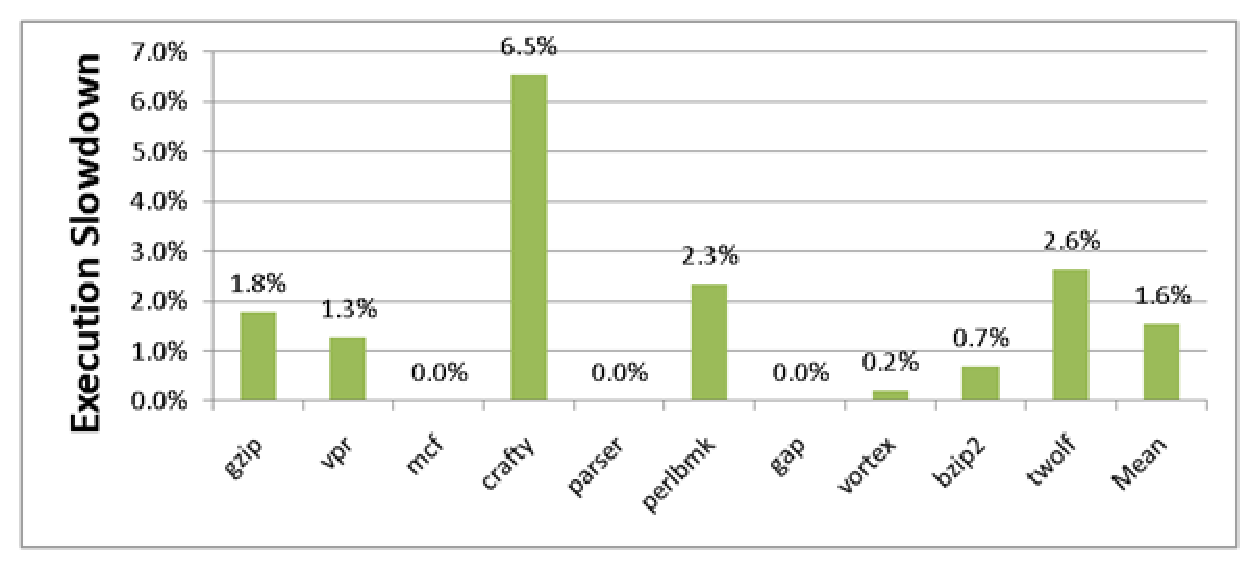
\includegraphics[scale=0.6]{relocperf.eps}
\caption{Application overhead caused by preparing the code for instrumentation but without
any instrumentation inserted.}
\end{figure}

The next set of experiments shows how much overhead is introduced due to counting the
basic block executions in the code. We use this particular instrumentation tool because basic block counting
is an example of an instrumentation tool where we would expect PIX to generate efficient instrumented executables
as the number of instrumentation points required is high. Much of the work performed in basic block counting, namely updating a single
counter every time a basic block is encountered, can be done easily using a fast instrumentation snippet rather than
by a full instrumentation function. The counters embodied in the instrumentation snippets must also be
persistent throughout the entire run of the application, which is more suited to a static instrumentation approach
because the static instrumentation does not utilize any resources to determine whether instrumentation can be removed.
The basic block counting instrumentation tool is used to produce an instrumented
executable for each program in our benchmark suite, whose runtime is compared to the runtime of the 
unmodified original executable. The results of these experiments are shown in Figure \ref{Figure:ToolOverheads}. 

\begin{figure}[ht]
\centering
\label{Figure:ToolOverheads}
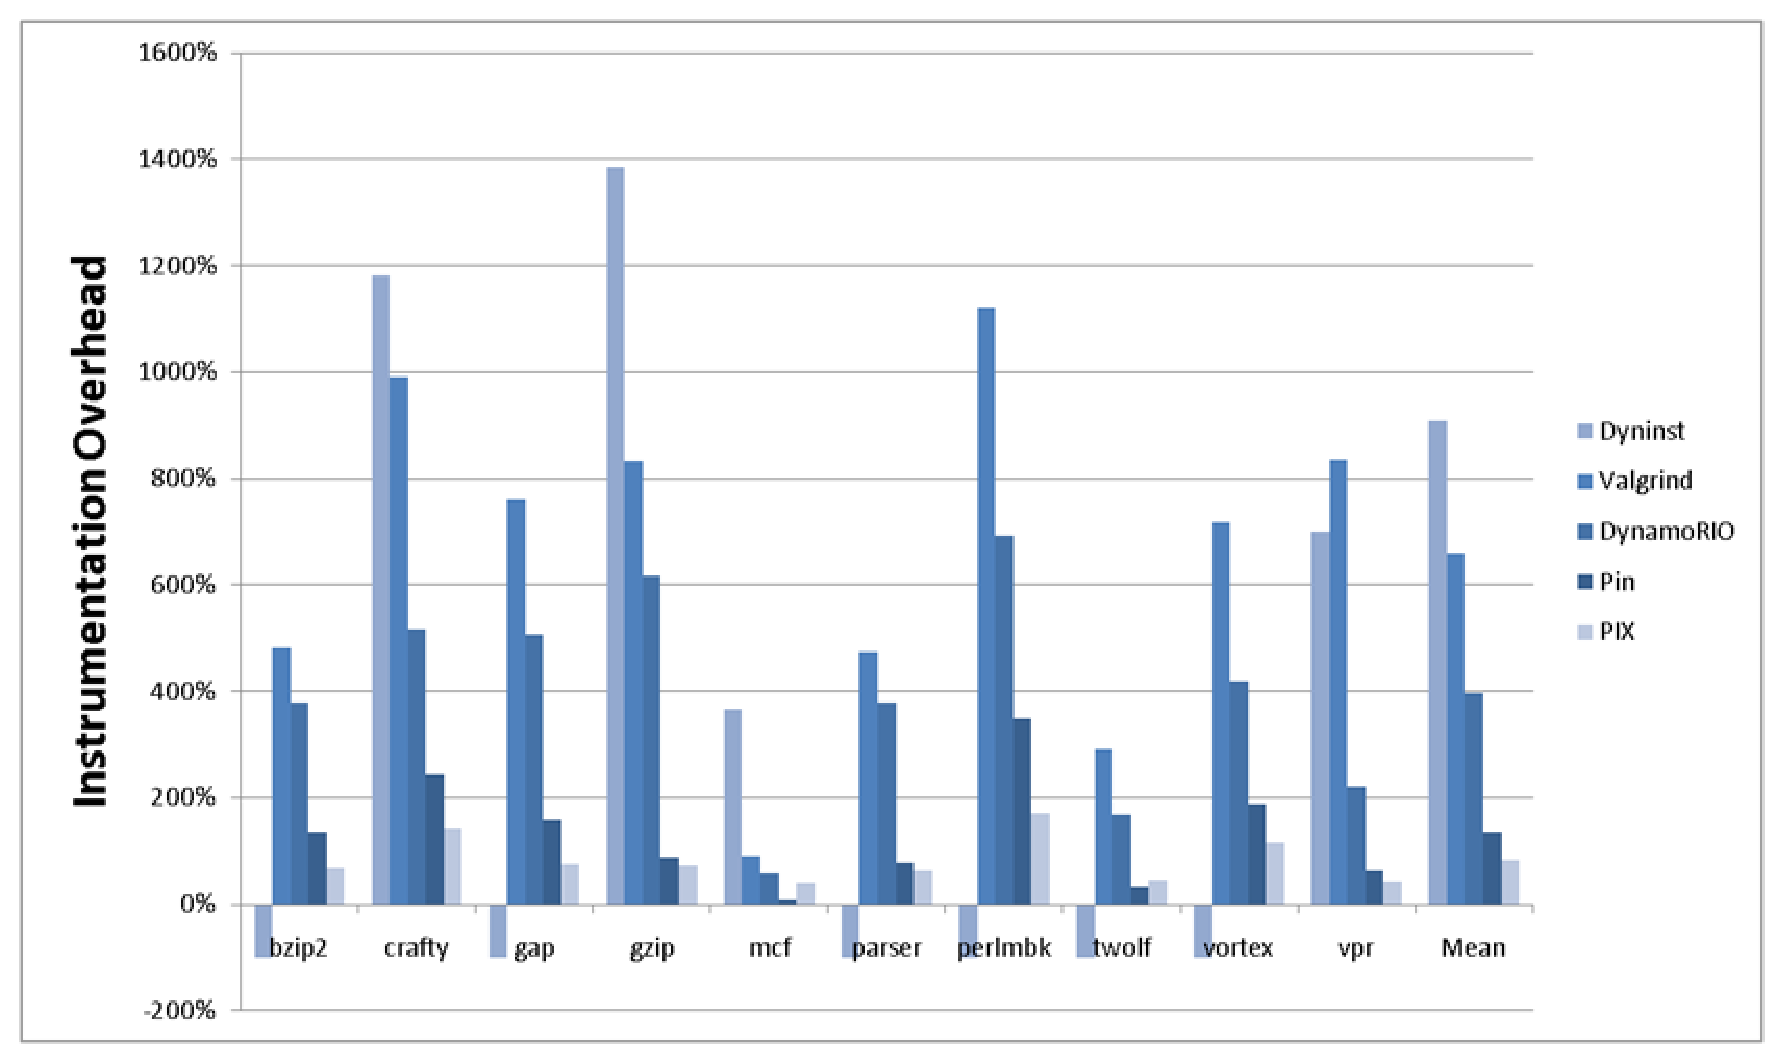
\includegraphics[scale=0.5]{bbcount.eps}
\caption{Performance of several x86 instrumentation tools with basic block counting instrumentation.}
\end{figure}

Figure \ref{Figure:ToolOverheads} presents the overhead introduced as a percentage of the original application runtime. The
overhead of PIX's basic block counter ranges from 41\%-170\% for the benchmakrs tested with an average overhead of 
84\%. More importantly, this figure shows that the overhead introduced by PIX instrumentation is significantly 
lower than those introduced by the other instrumentation toolkits available for the x86 platform. 
The average overhead is 135\% for Pin (ranging from 8\%-350\%), 
396\% for DynamoRIO (ranging from 58\%-693\%), 660\% for Valgrind (ranging from 91\%-1120\%), and XXX\% for Dyninst (ranging from 367\%-2079\%). 
Our experiments demonstrate that executables instrumented by PIX run an average of
51\% faster than the next most efficient instrumentation toolkit for basic block counting, Pin. Furthermore,
Pin uses a variety of optimizations such as tracking eflags bit liveness \cite{luk2005pin} that are currently
unincorporated into PIX. We plan to incorporate more optimizations to PIX in the future (see Section \ref{Section:Future}) including
several optimizations already in use by Pin, which should further improve the efficiency of the instrumented
executables generated by PIX.

